% Diagrama de arquitectura de Voctomix 2.0 — estilo formal
% Incluir desde main.tex con \input{figuras/diagrama_sistema}
% Compilar de forma independiente: pdflatex diagrama_sistema_standalone.tex

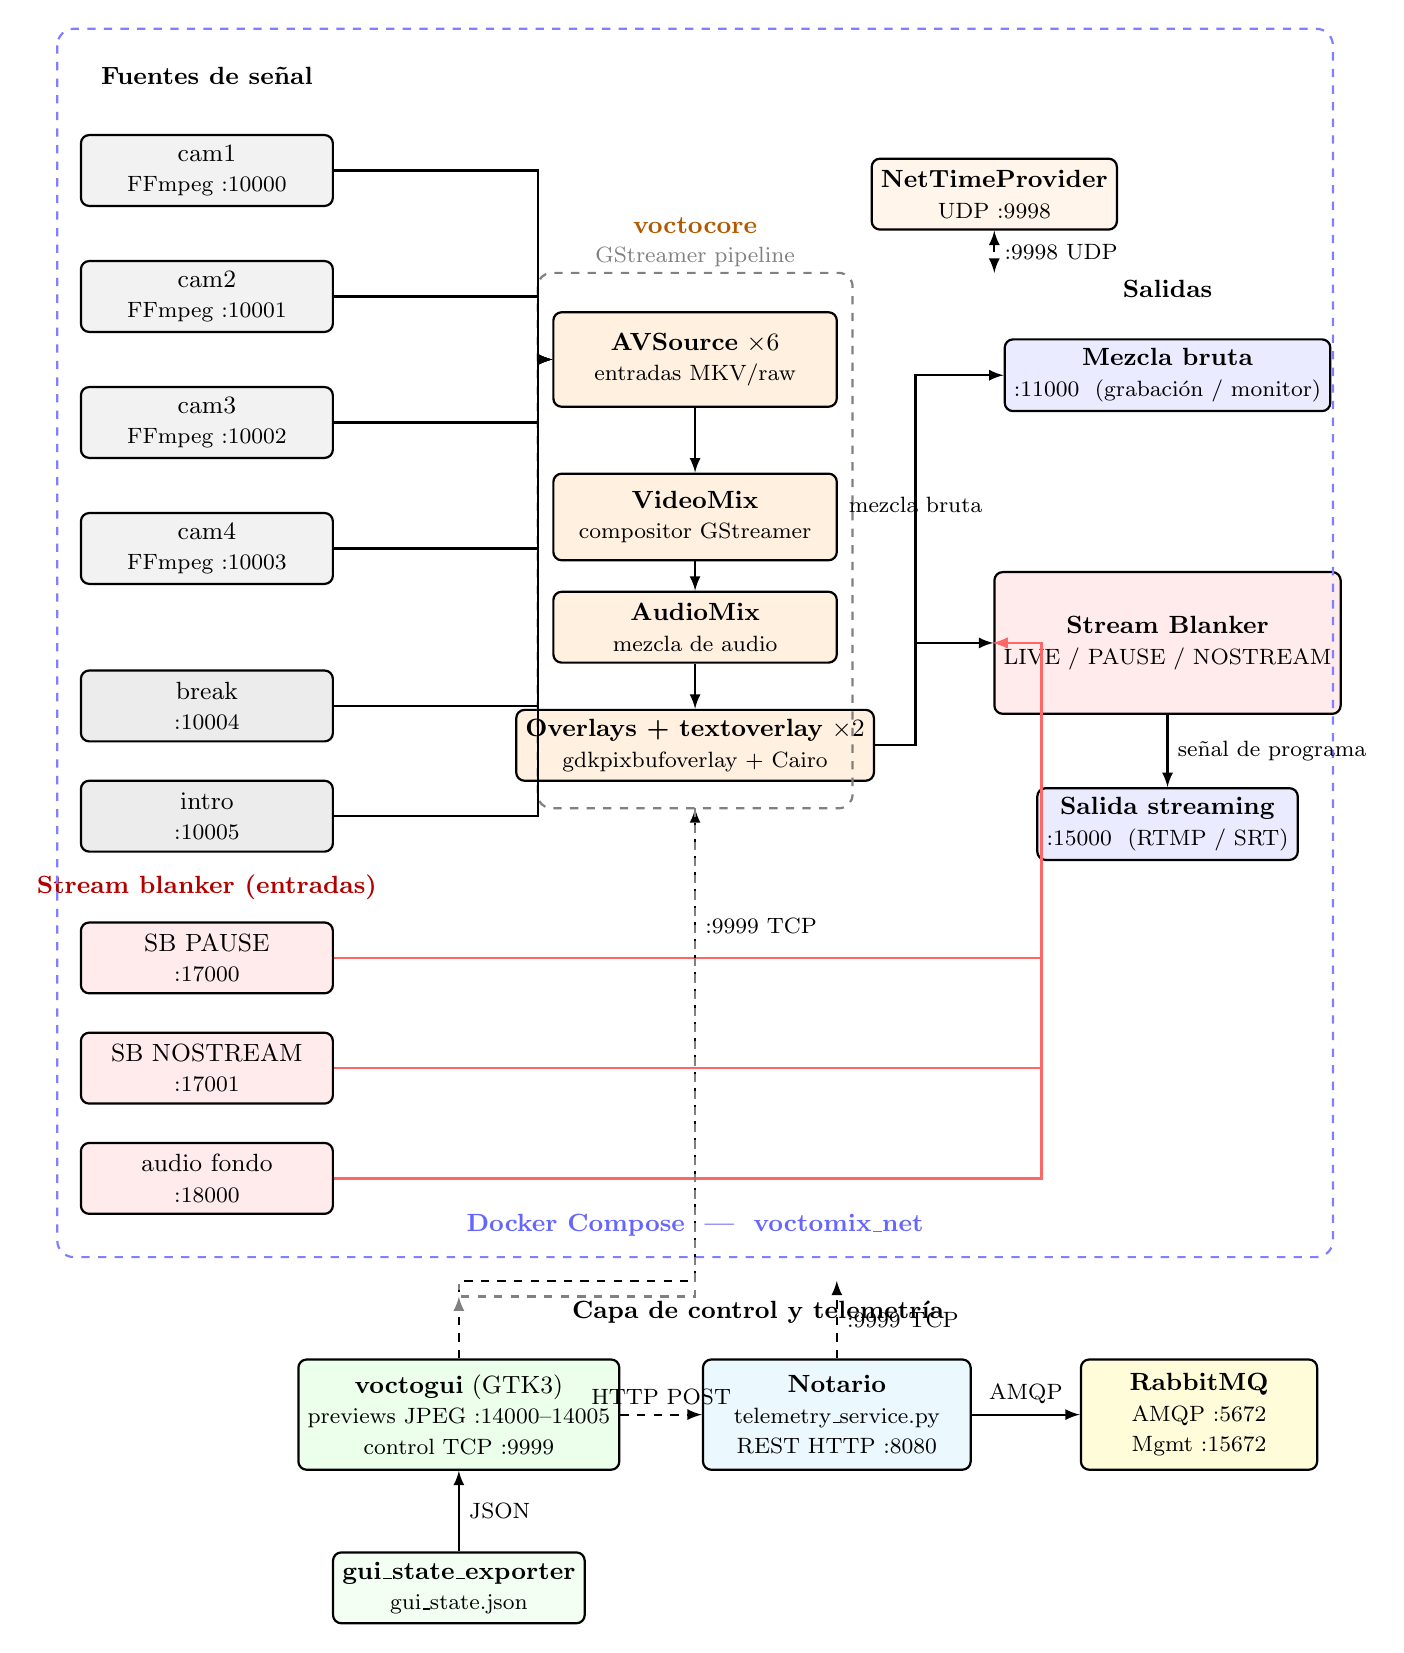
\begin{tikzpicture}[>=latex, thick, font=\small,
  box/.style={draw, rounded corners=3pt, align=center, minimum height=0.9cm},
  lbl/.style={font=\small\bfseries},
]

% ── anchuras de columna ──────────────────────────────────────────────────
% Col A (fuentes) x=0   Col B (voctocore) x=6   Col C (salidas) x=12

% ════════════════════════════════════════════════════════════════════════
%  COLUMNA A — Fuentes de señal
% ════════════════════════════════════════════════════════════════════════

% Cámaras
\node[box, minimum width=3.2cm, fill=gray!10] (cam1) at (0, 4.8)
  {cam1 \\ {\footnotesize FFmpeg :10000}};
\node[box, minimum width=3.2cm, fill=gray!10] (cam2) at (0, 3.2)
  {cam2 \\ {\footnotesize FFmpeg :10001}};
\node[box, minimum width=3.2cm, fill=gray!10] (cam3) at (0, 1.6)
  {cam3 \\ {\footnotesize FFmpeg :10002}};
\node[box, minimum width=3.2cm, fill=gray!10] (cam4) at (0, 0)
  {cam4 \\ {\footnotesize FFmpeg :10003}};

% Auxiliares
\node[box, minimum width=3.2cm, fill=gray!15] (brk) at (0,-2.0)
  {break \\ {\footnotesize :10004}};
\node[box, minimum width=3.2cm, fill=gray!15] (intro) at (0,-3.4)
  {intro \\ {\footnotesize :10005}};

% Stream blanker inputs
\node[box, minimum width=3.2cm, fill=red!8] (sbp) at (0,-5.2)
  {SB PAUSE \\ {\footnotesize :17000}};
\node[box, minimum width=3.2cm, fill=red!8] (sbn) at (0,-6.6)
  {SB NOSTREAM \\ {\footnotesize :17001}};
\node[box, minimum width=3.2cm, fill=red!8] (sba) at (0,-8.0)
  {audio fondo \\ {\footnotesize :18000}};

% Etiquetas de grupo col A
\node[lbl] at (0, 6.0)  {Fuentes de señal};
\node[lbl, text=red!70!black] at (0,-4.3) {Stream blanker (entradas)};

% ════════════════════════════════════════════════════════════════════════
%  COLUMNA B — voctocore (núcleo GStreamer)
% ════════════════════════════════════════════════════════════════════════

\node[box, minimum width=3.6cm, minimum height=1.2cm, fill=orange!12] (avsrc) at (6.2, 2.4)
  {\textbf{AVSource} $\times$6 \\ {\footnotesize entradas MKV/raw}};

\node[box, minimum width=3.6cm, minimum height=1.1cm, fill=orange!12] (vmix) at (6.2, 0.4)
  {\textbf{VideoMix} \\ {\footnotesize compositor GStreamer}};

\node[box, minimum width=3.6cm, fill=orange!12] (amix) at (6.2,-1.0)
  {\textbf{AudioMix} \\ {\footnotesize mezcla de audio}};

\node[box, minimum width=3.6cm, fill=orange!12] (ovl) at (6.2,-2.5)
  {\textbf{Overlays + textoverlay} $\times$2 \\ {\footnotesize gdkpixbufoverlay + Cairo}};

% Borde contenedor voctocore
\draw[rounded corners=5pt, dashed, gray]
  (4.2, 3.5) rectangle (8.2,-3.3);
\node[lbl, text=orange!70!black] at (6.2, 4.1) {voctocore};
\node[font=\footnotesize, text=gray] at (6.2, 3.7) {GStreamer pipeline};

% flechas internas voctocore
\draw[->] (avsrc.south) -- (vmix.north);
\draw[->] (vmix.south)  -- (amix.north);
\draw[->] (amix.south)  -- (ovl.north);

% ════════════════════════════════════════════════════════════════════════
%  COLUMNA C — Stream blanker y salidas
% ════════════════════════════════════════════════════════════════════════

\node[box, minimum width=3.2cm, minimum height=1.8cm, fill=red!8] (sb) at (12.2, -1.2)
  {\textbf{Stream Blanker} \\ {\footnotesize LIVE / PAUSE / NOSTREAM}};

\node[box, minimum width=3.2cm, fill=blue!8] (outraw) at (12.2, 2.2)
  {\textbf{Mezcla bruta} \\ {\footnotesize :11000 \ (grabación / monitor)}};

\node[box, minimum width=3.2cm, fill=blue!8] (outst) at (12.2,-3.5)
  {\textbf{Salida streaming} \\ {\footnotesize :15000 \ (RTMP / SRT)}};

\node[lbl] at (12.2, 3.3) {Salidas};

% ════════════════════════════════════════════════════════════════════════
%  FILA INFERIOR — GUI, Notario, RabbitMQ
% ════════════════════════════════════════════════════════════════════════

\node[box, minimum width=4.0cm, minimum height=1.4cm, fill=green!8] (gui) at (3.2,-11.0)
  {\textbf{voctogui} (GTK3) \\ {\footnotesize previews JPEG :14000--14005} \\
   {\footnotesize control TCP :9999}};

\node[box, minimum width=3.4cm, minimum height=1.4cm, fill=cyan!8] (notario) at (8.0,-11.0)
  {\textbf{Notario} \\ {\footnotesize telemetry\_service.py} \\
   {\footnotesize REST HTTP :8080}};

\node[box, minimum width=3.0cm, minimum height=1.4cm, fill=yellow!15] (rmq) at (12.6,-11.0)
  {\textbf{RabbitMQ} \\ {\footnotesize AMQP :5672} \\
   {\footnotesize Mgmt :15672}};

\node[lbl] at (7.0,-9.7) {Capa de control y telemetría};

% gui_state_exporter
\node[box, minimum width=3.0cm, fill=green!5] (gse) at (3.2,-13.2)
  {\textbf{gui\_state\_exporter} \\ {\footnotesize gui\_state.json}};

% NetTimeProvider
\node[box, minimum width=2.8cm, fill=orange!8] (ntp) at (10.0, 4.5)
  {\textbf{NetTimeProvider} \\ {\footnotesize UDP :9998}};

% ════════════════════════════════════════════════════════════════════════
%  BORDE DOCKER
% ════════════════════════════════════════════════════════════════════════
\draw[rounded corners=6pt, dashed, blue!50, line width=0.8pt]
  (-1.9, 6.6) rectangle (14.3,-9.0);
\node[font=\small\bfseries, text=blue!60] at (6.2,-8.6)
  {Docker Compose \ — \ voctomix\_net};

% ════════════════════════════════════════════════════════════════════════
%  FLECHAS — fuentes → voctocore
% ════════════════════════════════════════════════════════════════════════
% cámaras → avsrc (recogen en punto intermedio x=4.2)
\foreach \cam/\y in {cam1/4.8, cam2/3.2, cam3/1.6, cam4/0}{
  \draw[->] (\cam.east) -- (4.2,\y) -- (4.2, 2.4) -- (avsrc.west |- {(0,2.4)});
}
% auxiliares → avsrc
\draw[->] (brk.east)  -- (4.2,-2.0) -- (4.2, 2.4) -- (avsrc.west |- {(0,2.4)});
\draw[->] (intro.east) -- (4.2,-3.4) -- (4.2, 2.4) -- (avsrc.west |- {(0,2.4)});

% ovl → bifurcación derecha
\coordinate (oveast) at (9.0,-2.5);
\draw[->] (ovl.east) -- (oveast) |- (outraw.west)
  node[pos=0.3, above, font=\footnotesize] {mezcla bruta};
\draw[->] (oveast) |- (sb.west);

% SB inputs → sb
\draw[->, red!60] (sbp.east) -- (10.6,-5.2) |- (sb.west);
\draw[->, red!60] (sbn.east) -- (10.6,-6.6) |- (sb.west);
\draw[->, red!60] (sba.east) -- (10.6,-8.0) |- (sb.west);

% sb → salida streaming
\draw[->] (sb.south) -- (outst.north)
  node[midway, right, font=\footnotesize] {señal de programa};

% ════════════════════════════════════════════════════════════════════════
%  FLECHAS — control y telemetría
% ════════════════════════════════════════════════════════════════════════
% gui → voctocore
\draw[->, dashed] (gui.north) -- (3.2,-9.3) -- (6.2,-9.3) -- (6.2,-3.3)
  node[near end, right, font=\footnotesize] {:9999 TCP};

% notario → voctocore
\draw[->, dashed] (notario.north) -- (8.0,-9.3)
  node[midway, right, font=\footnotesize] {:9999 TCP};

% gui_state_exporter → gui
\draw[->] (gse.north) -- (gui.south)
  node[midway, right, font=\footnotesize] {JSON};

% gui → notario (HTTP POST)
\draw[->, dashed] (gui.east) -- (notario.west)
  node[midway, above, font=\footnotesize] {HTTP POST};

% notario → rabbitmq
\draw[->] (notario.east) -- (rmq.west)
  node[midway, above, font=\footnotesize] {AMQP};

% ntp ↔ voctocore
\draw[<->, dashed] (ntp.south) -- (ntp.south |- {(0,3.5)})
  node[midway, right, font=\footnotesize] {:9998 UDP};

% previews gui
\draw[->, dashed, gray] (6.2,-3.3) -- (6.2,-9.5) -- (3.2,-9.5) -- (gui.south |- {(0,-9.5)});

\end{tikzpicture}
